\documentclass{ar2rc}

\usepackage{graphicx}
\usepackage{beraserif}
\usepackage{natbib}

\title{An Improved Minimum-Distance Texture Estimator for Speckled Data under the $\mathcal{G}^0$ Model}
\author{Julia~Cassetti,
	Alejandro~C.~Frery}
\journal{Journal of Mathematical Imaging and Vision}
%\doi{12345}

\begin{document}
	
	\maketitle
	
	\section{Reviewer \#1}
	
	\subsection{Summary}
	
\fbox{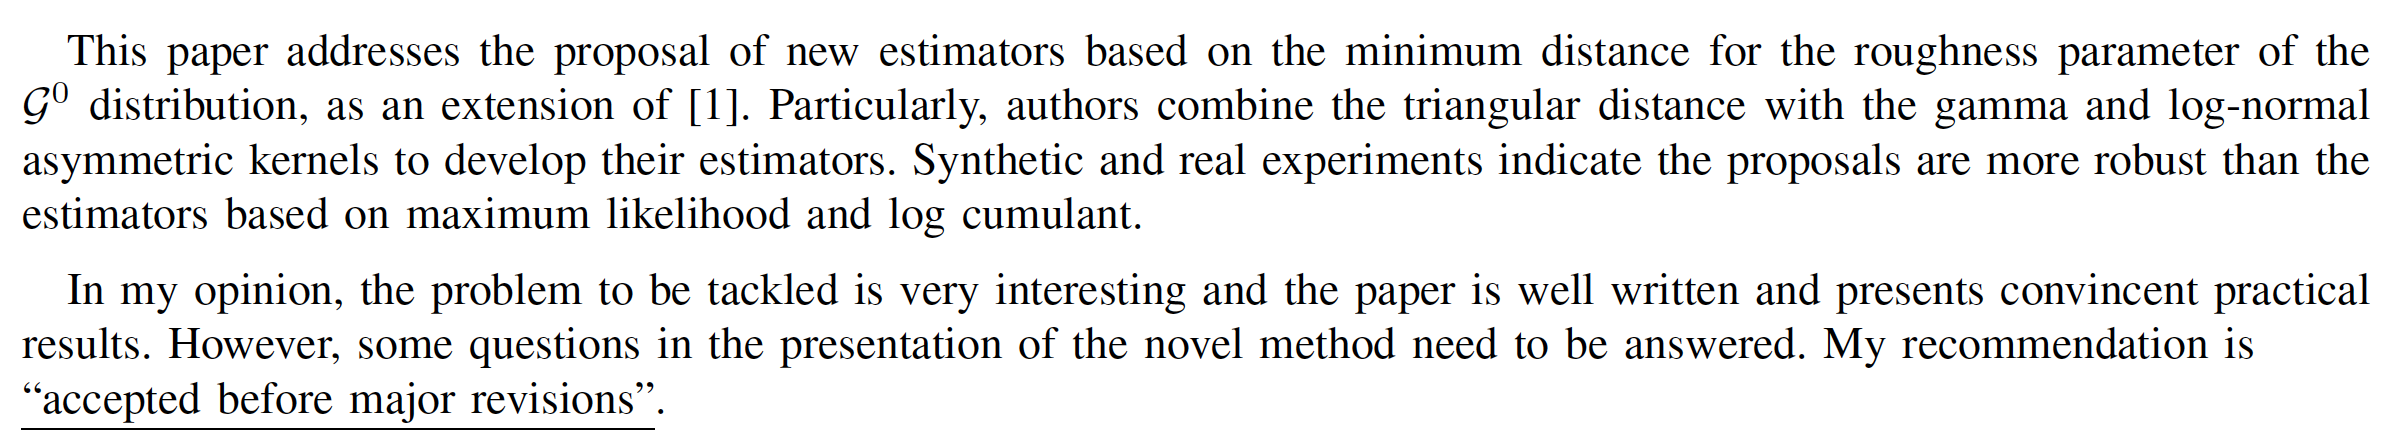
\includegraphics[width=\linewidth]{Summary}}	

\AR We would like to thank the reviewer for the careful analysis of our work.
We agree with the suggestions, and we have proceeded accordingly.
	
	\subsection{Critical comments}

\fbox{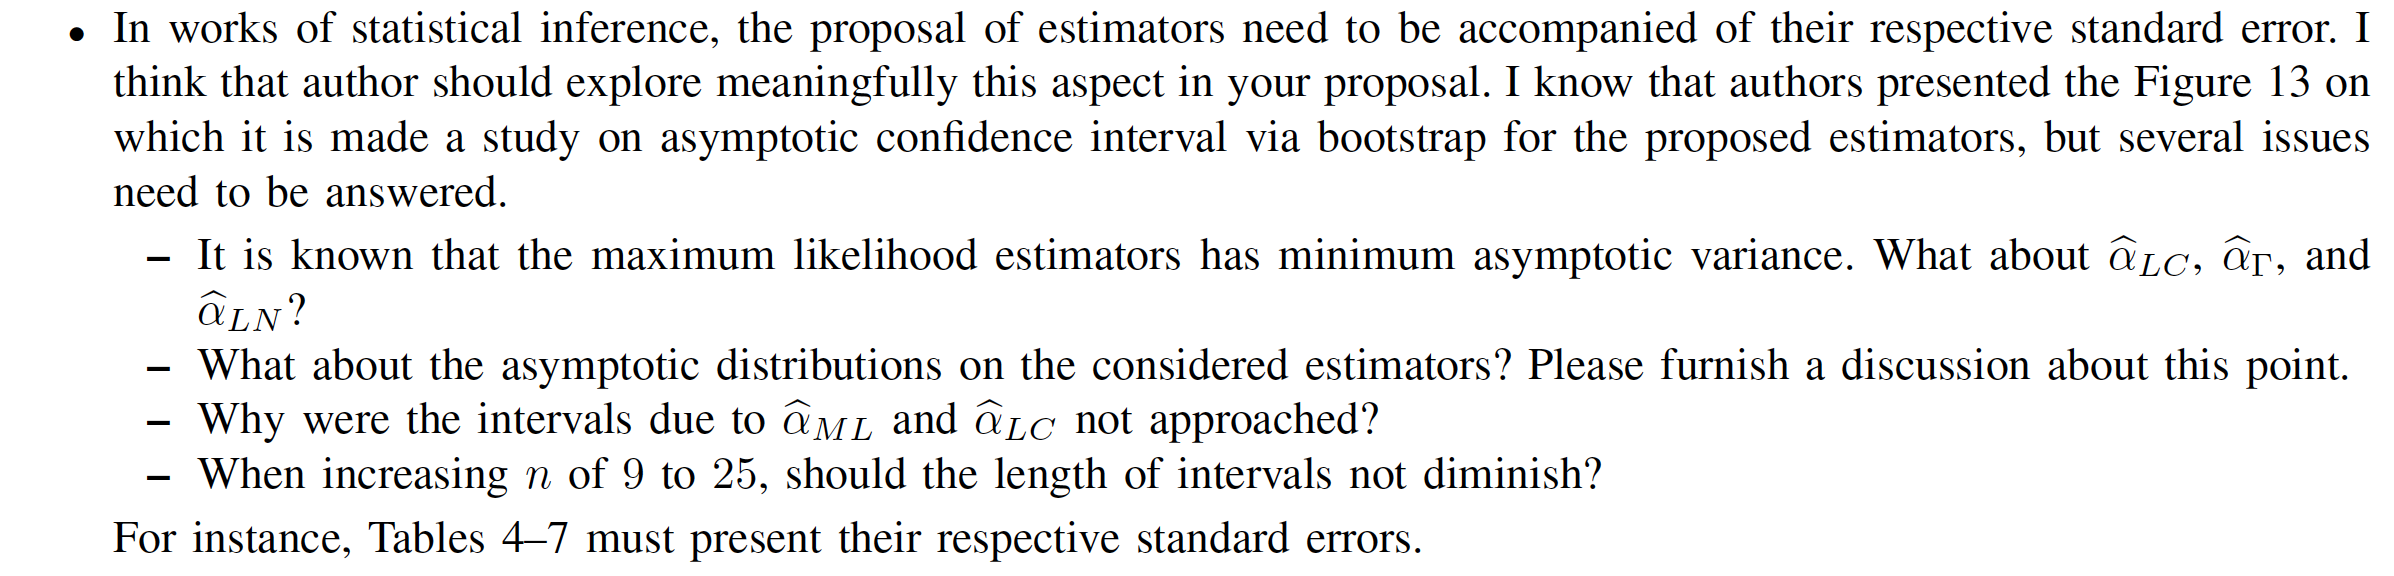
\includegraphics[width=\linewidth]{Critical}}
	
\subsection{Detailed comments}

\fbox{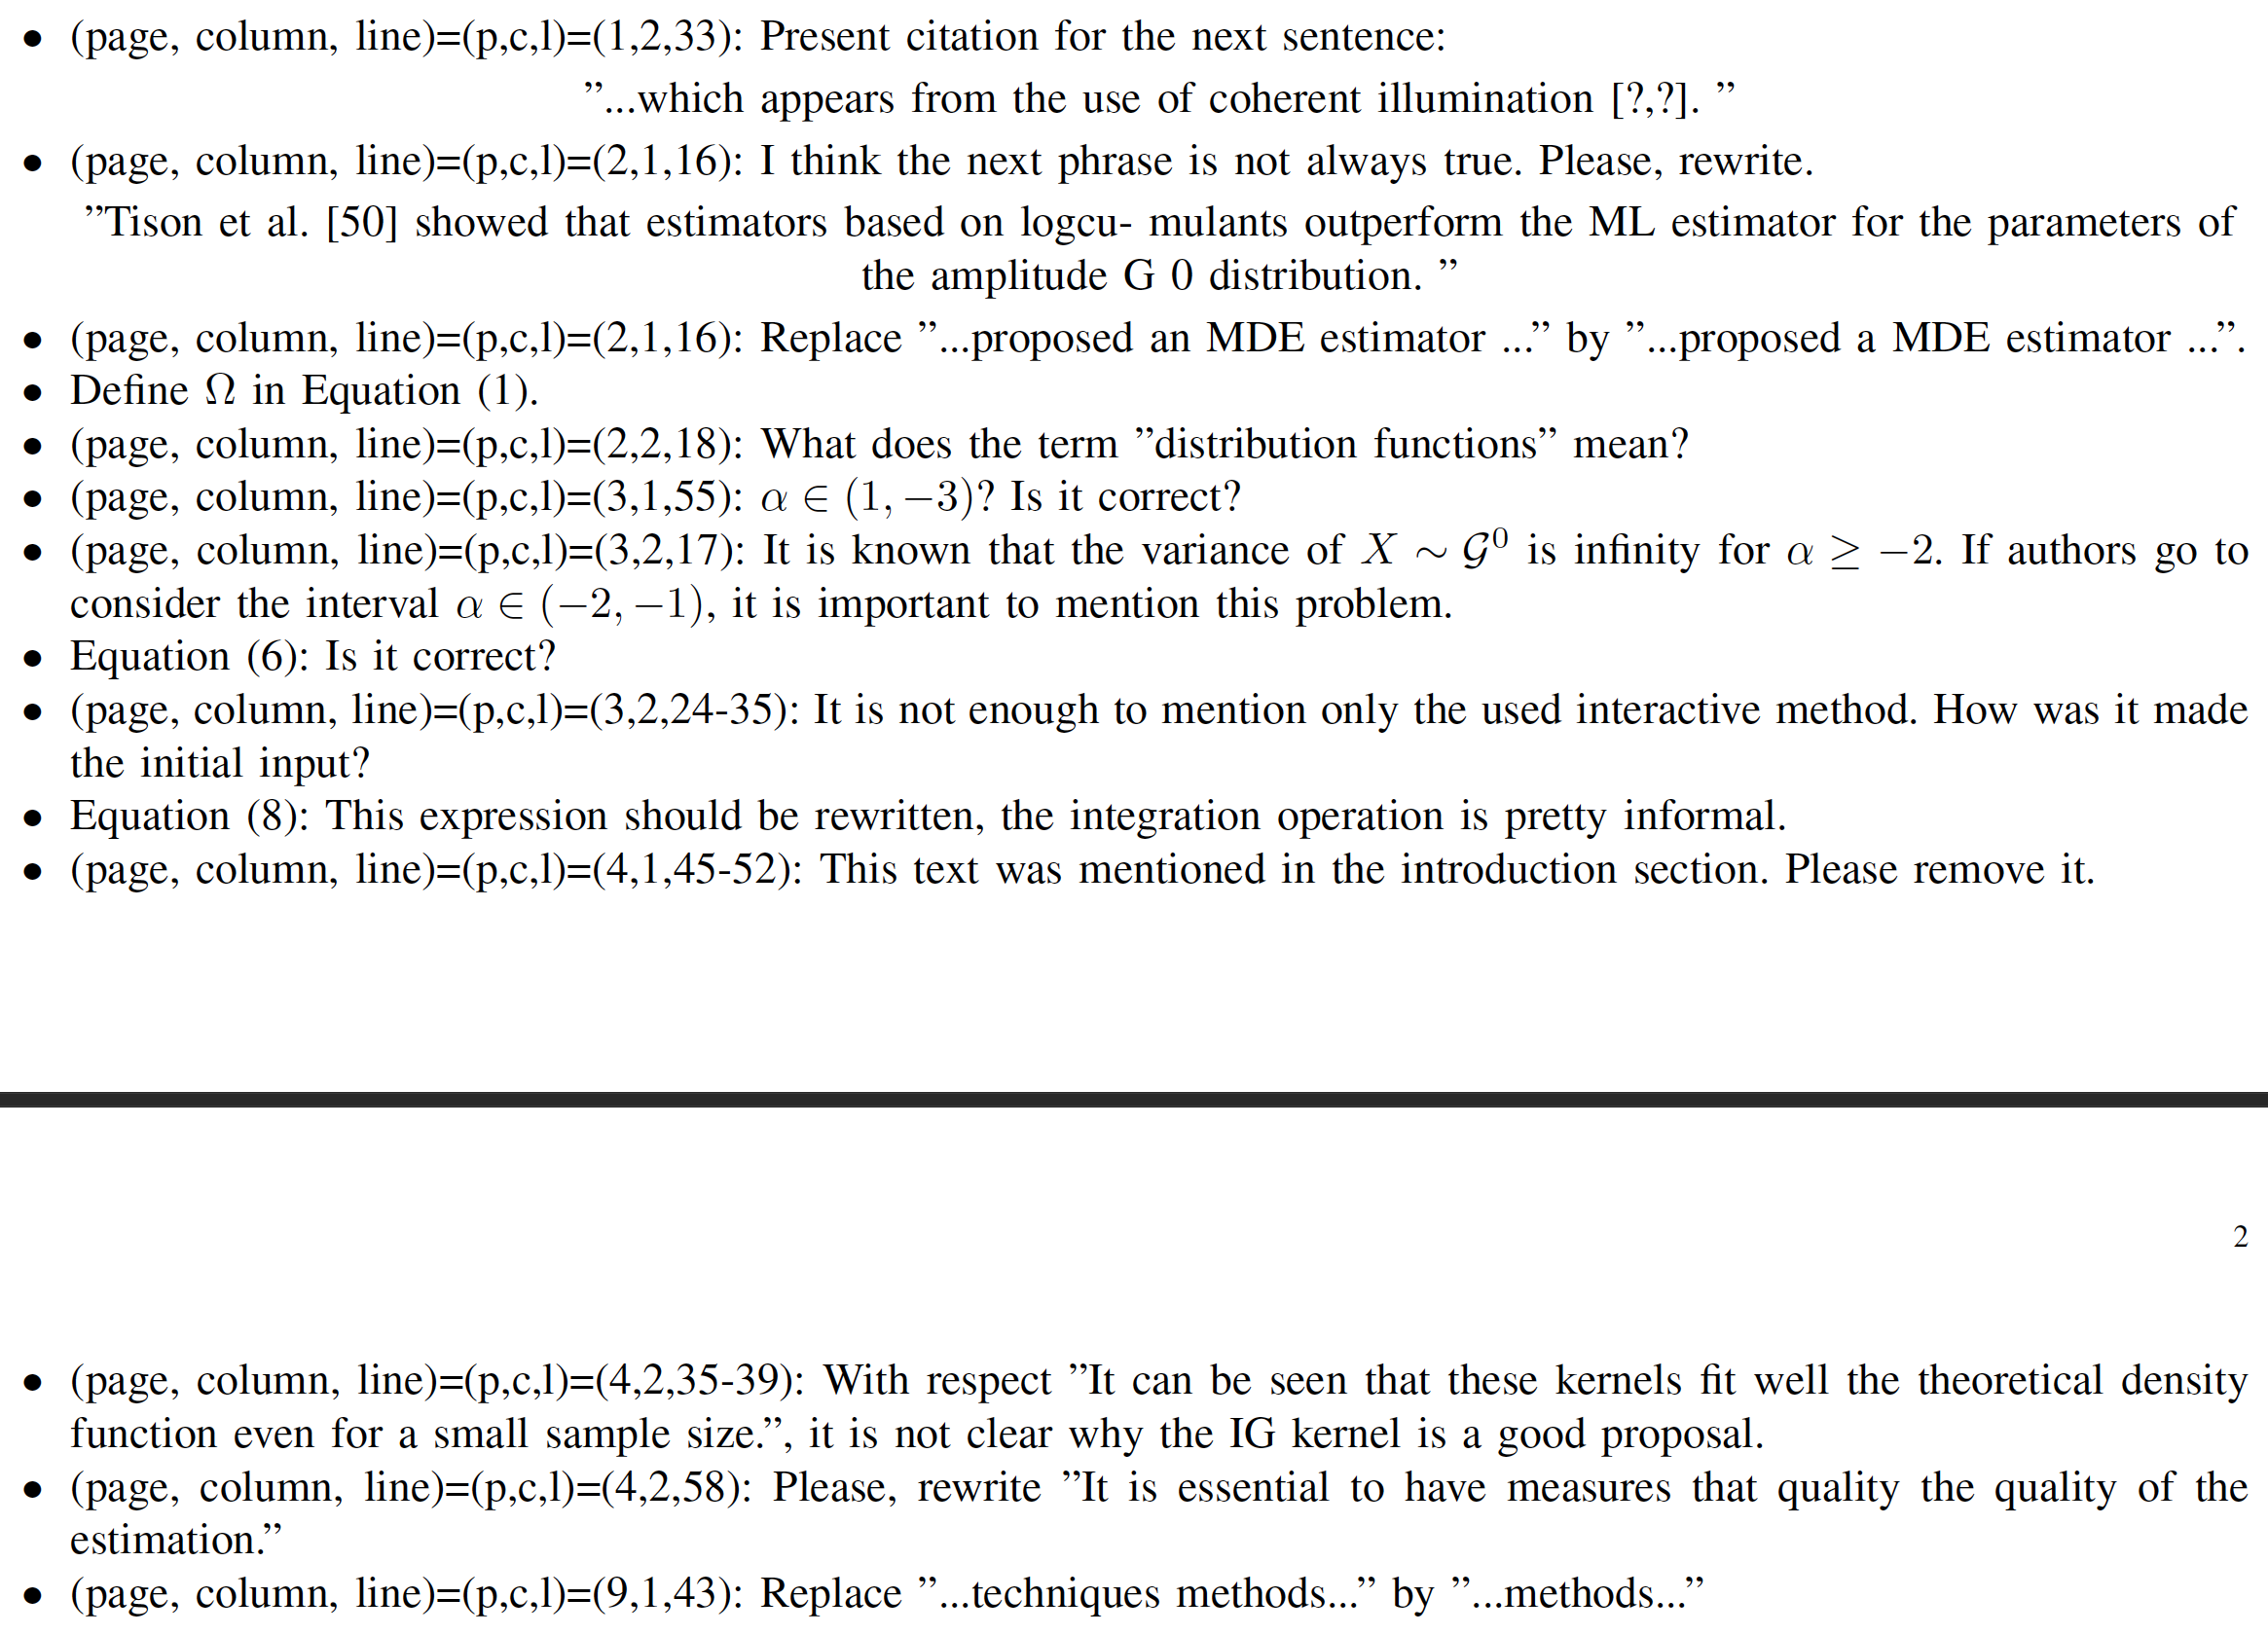
\includegraphics[width=\linewidth]{Detailed}}

\AR We have made the following changes:
\begin{itemize}
\item We have added the reference by \citet{SARImageStatisticalModelingPartISinglePixelStatisticalModels}, which is a modern and comprehensive survey about speckle.
\item 
\item 
\item We added ``and $\Omega$ is the parameter space.'' to the sentence after~(1).
\item We changed the text as follows
		\begin{quote}
	In particular, several measures have been proposed to reflect the closeness  \DIFdelbegin \DIFdel{between two distribution functions.} \DIFdelend \DIFaddbegin \DIFadd{among the models that describe samples.}\DIFaddend
		\end{quote}
\item It was wrong; we corrected it and now it reads ``$\alpha \in (-1,-3)$''.
\item 
\item 
\item 
\item We changed the text as follows:
	\begin{quote}		
	It is essential to have measures that \DIFdelbegin \DIFdel{quality} \DIFdelend \DIFaddbegin \DIFadd{quantify }\DIFaddend the quality of the estimation. 
	\end{quote}
\item We deleted the word ``techniques''.
\end{itemize}

\bibliographystyle{agsm}
\bibliography{../../../../../Bibliography/bib_julia2}
	
\end{document}
